\documentclass[12pt]{article}

\usepackage[T1]{fontenc}
\usepackage{a4wide}
\usepackage{mathptmx}
\usepackage{graphicx}
\usepackage[hidelinks]{hyperref}
\usepackage{mathbbol,bm,amsmath,amsthm,amsfonts,amssymb}
\usepackage{mathtools}
\usepackage{booktabs}
\usepackage{fancybox}
\usepackage[shortlabels]{enumitem}
\usepackage{tikz}
\usepackage{nicefrac}
\usepackage{fancyhdr}

\setlist[itemize]{label={$\bullet$}, topsep=-0.2ex,
  partopsep=0pt, parsep=4pt, itemsep=0pt, leftmargin=4.5mm,
  labelsep=0.5ex}

\setlist[enumerate]{align=left, listparindent=0pt}

\newcommand{\R}{\mathbb{R}}
\newcommand{\N}{\mathbb{N}}
\newcommand{\Z}{\mathbb{Z}}
\renewcommand{\iff}{\;\leftrightarrow\;}
\newcommand{\floor}[1][x]{\lfloor #1\rfloor}
\newcommand{\ceil}[1][x]{\lceil #1\rceil}
\newcommand{\mat}[1][A]{\text{\textbf{#1}}}
\newcommand{\I}{\mathbb{1}}

\makeatletter
\newcommand*{\bdiv}{%
  \nonscript\mskip-\medmuskip\mkern5mu%
  \mathbin{\operator@font div}\penalty900\mkern5mu%
  \nonscript\mskip-\medmuskip
}
\makeatother

\renewcommand{\thesubsection}{\arabic{subsection}}
\renewcommand{\thesubsubsection}{\alph{subsubsection}}

\pagestyle{fancy}
\fancyhf{}
\rhead{\textbf{Alexander Bergenholtz} \\ Compulsory Assignment 5}
\lhead{MNF130}
\chead{\today}


\setlength{\parindent}{0pt}
\setlength{\parskip}{1ex plus 0.5ex minus 0.2ex}

\newenvironment{answer}{\color{blue}}{}
\newcommand{\bl}[1][T]{{\color{blue}#1}}

\graphicspath{{./}{../images/}}

\title{\huge Compulsory Assignment 5}

\author{\LARGE MNF130V2020}

\date{\Large\textbf{Due on: Sunday 3 May 2020, 23:59}}


\begin{document}

\maketitle

\bigskip

  \vspace*{15mm}

  {\large
  \begin{minipage}{\linewidth}
    \begin{itemize}
    \item Submit your assignment as a \textbf{single PDF file}.
      \smallskip
    \item You can write your assignment in \LaTeX, using the template
      provided, or by hand.
      \smallskip
    \item For hand-written submission, use a scanner or high-quality
      scanning app on your phone.
      \smallskip
    \item Write your answers \textbf{one-sided} (don't use both sides
      of a page), and start a new page for every exercise.
      \smallskip
    \item You may write your answers in English or Norwegian.
      \smallskip
    \item The assignment covers the syllabus from Rosen Section 5.3 to
      Section 10.3.
      \smallskip
    \item The assignment is scored on \textbf{24 points}. Hence you
      need to score \textbf{at least 8.5 points to pass}.
  \end{itemize}
  \end{minipage}
  }

\bigskip

\bigskip

\newpage

\subsection{Recursion and structural induction (7 points)}

The set of full binary trees is defined recursively by:
\begin{itemize}
\item \emph{Basis step:} There is a full binary tree consisting of a
  single vertex $r$.
\item \emph{Recursive step:} If $T_1$ and $T_2$ are disjoint full
  binary trees, then the tree $T=T_1\cdot T_2$ formed by connecting
  a new root $r$ to each of the roots of the left subtree $T_1$ and
  right subtree $T_2$ is also a full binary tree.
\end{itemize}

\begin{enumerate}[a)]
\item Give recursive definitions of the functions $n(T)$ and $\ell(T)$
  which count the number of vertices and the number of leaves,
  respectively, in a full binary tree. (\textbf{Hint:} A recursive
  definition of the set of leaves of a full binary tree can be found
  in Rosen Chapter 5!)
  \medskip

  \begin{itemize}
  \item Since the is a full binary tree, the number of vertices will be $T_1 + T_2 + 1$, where $T_1,T_2$ are children sub-trees of the root vertex and the $1$ is the root vertex itself. Hence: \\

    \textit{Basis step:} The full binary tree consisting of a single vertex \textit{r} has $n(T)=1$. \\
    \textit{Recursive step:} $T = T_1 \cdot T_2$ where $T_1,T_2$ are sub(full-binary)trees from the root vertex $r$.  The number of vertices at step \textit{n} becomes: \\
      $$
  n(T) = 1 + n(T_1) + n(T_2)
  $$
  \qed 
\item
  \textit{Basis step:} The root vertex \textit{r} is a leaf and a full binary tree consisting of that single vertex, such that $l(T) = 1$. \\
  \textit{Recursive step:} The leaves for the tree $T = T_1 \cdot T_2$ where $T_1,T_2$ are subtrees of the root \textit{r} such that the total number of leaves in the tree becomes the union of $T_1$ and $T_2$. \\
  $$
  \ell(T) = \ell(T_1) + \ell(T_2)
  $$ 

  \end{itemize}

\qed
\item  Prove that $n(T)=2\ell(T)-1$ for all full binary trees $T$,
  using structural induction.

  \begin{itemize}
  \item From part \textit{a)}, we found that $n(T) = 1 + n(T_1) + n(T_2)$. Now if $n(T) = 2 \ell(T) -1$, we can rewrite it as: \\
    $$
    n(T) = 1 + (2\ell(T_1) - 1) + (2\ell(T_2) - 1) 
    $$

    Now let $P(T) = (n(T) = 2\ell(T) -1)$ \\ 
    
    The basis step $n(T) = 1$ which implies $\ell(T) = 1$: \\
    $$
    1 =  2\cdot1 - 1 = 2 - 1 = 1
    $$

    Such that $P(T)$ is true. \\

    Now we assume it to be true for $P(T_1),P(T_2)$, where $T_1,T_2$  being two full binary trees, such that: \\

    $$
    n(T) = n(T_1 \cdot T_2) = 1 + (2\ell(T_1) -1) + (2\ell(T_2) -1)
    $$
    $$
    = (2\ell(T_1) + 2\ell(T_2)) - 1
    $$
    $$
    = 2\ell(T_1 + T_2) - 1
    $$
    Such that $P(T)$ is true for all $T$ by structural induction.
    \qed
    
    
  \end{itemize}

  
 \end{enumerate}

 \bigskip
 \newpage

\subsection{Counting (6 points)}
\label{sec:counting}

A standard deck of cards contains 52 cards: 13 cards each of 4
different ``suits'', hearts (red), diamonds (red), spades (black) and
clubs (black).

\begin{enumerate}[a)]
\item How many cards must be selected from a standard deck of cards to
  guarantee that at least 3 cards of the same suit are selected?
  Explain your answer.

  \begin{itemize}
  \item By the pigeonhole principle, we have four boxes, one for each suit. In order to have two of the same suit, we have to draw 5 cards, since the fifth card will ensure a repetition of one of the suits. To guarantee at least three of the same suit, we have to draw 9 cards. With 9 cards, one of the four boxes will have at least 3 cards in it, thus satisfying the criteria.
  \end{itemize}
  \qed
  \medskip
  

\item How many ways are there to select a pair of cards from a
  standard deck of cards such that one of the cards is red and the
  other one is black? Your answer can contain factorial or power
  expressions. Explain your answer.

  \begin{itemize}
  \item We have 26 black cards and 26 red cards and amongst these we have $26 \cdot 26$ possibilities, because for each black card there are 26 red cards to choose from, and vice versa. \\
    The number of ways to select a red and then a black card becomes: \\
    $$26\cdot 26 = 26^2 $$

    
  \end{itemize}
  \qed

\medskip


\item How many ways are there to divide a standard deck of cards over
  4 players? Your answer can contain factorial or power
  expressions. Explain your answer.

  \begin{itemize}
  \item To divide the deck of cards equally, each player gets 13 cards. We hand out 13 cards to the first player, which means selecting 13 cards from the deck of 52, which gives us $C(52,13)$. \\
    Subtracting those 13 cards, the new number of possibilities of cards for the second player becomes $C(39,13)$. \\
    Repeat for the third player with $C(26,13)$. \\
    Finally, for the fourth player we get $C(13,13) = 1$. Multiplying this together, we get: \\

    $$
    \frac{52!}{13!39!} \cdot \frac{39!}{13!26!} \cdot \frac{26!}{13!13!} \cdot 1 = \frac{52!}{(13!)^4}
    $$

    
  \end{itemize}
  \qed

\end{enumerate}

\bigskip
\newpage

\subsection{Relations (6 points)}
\label{sec:relations}

\begin{enumerate}[a)]
\item Let $R$ be a binary relation on the set of integers such that
  $(a,b)\in R$ if and only if $b-a=1$. What is the composite relation
  $R\circ R$?

  \textit{Note that since the problem uses the set of integers, I interpret this as operating on $\mathbb{Z}$}.
  
  \begin{itemize}
  \item We can re-write the binary relation as: \\
    $$
    b - a = 1 \Rightarrow R = \{a,a+1 | a \in \mathbb{Z}\}
    $$
    and write the composite relation as: \\
    $$
    R \circ R = R^2
    $$

    In order for the relation $R^2$ to exist, we must have: 
    $$
    (a,c) \in R^2 \iff \exists b \rightarrow (a,b) \in R \wedge (b,c) \in R
    $$

    Now, since $R = \{a, a+1\}$ and $\{c = a + 2\}$, $R^2$ becomes: \\

    $$
    R \circ R = R^2 = \{a,b | a,b \in \mathbb{Z}, b - a = 2\}
    $$
    
  \end{itemize}
  \qed
  
\medskip

\item Let $R$ be a binary relation on the set of ordered pairs of
  integers such that $\bigl((a,b),(c,d)\bigr)\in R$ if and only if
  $b-a=d-c$. Show that $R$ is an equivalence relation.

  \begin{itemize}
  \item In order to show that $R$ is an equivalence relation, we must show that $R$ is reflexive, symmetric and transitive.
    \begin{itemize}
    \item $R$ is reflexive: We have to show that $(a,b)R(a,b)$. $b - a = b - a$ such that by definition of $R$, $(a,b)R(a,b)$. So $R$ is reflexive.
    \item $R$ is symmetric: We have the pairs $(a,b),(c,d)$ such that $(a,b)R(c,d)$. Now we must show that in order for $R$ to be symmetric,
      $(c,d)R(a,b)$. \\
      $(a,b)R(c,d)\Rightarrow b-a=d-c$. This implies that $d-c=b-a$ such that $(c,d)R(a,b)$ and thus $R$ is symmetric.
    \item $R$ is transitive: $(a,b)$ and $(c,d)$ are two ordered pairs. Suppose another ordered pair of integers $(e,f)$ such that $(a,b)R(c,d)$ and $(c,d)R(e,f)$.  We must now show that $(a,b)R(e,f)$. \\
      $(a,b)R(c,d) \Rightarrow b - a = d -c $ means that $c - d = a - b$ such that: \\ $(c,d)R(e,f)$ is $c - d = e - f$. This makes $a - b = e - f$, rewritten to:\\
      $f - e  = b - a$ which through the symmetric property implies $b - a = f - e$ and shows that $R$ is also transitive, which makes $R$ an equivalence relation. 
    \end{itemize}
  \end{itemize}
\end{enumerate}

\qed 
\bigskip
\newpage


\subsection{Graphs (5 points)}
\label{sec:graphs}

For the undirected graph shown, give the number of vertices, the
  number of edges, and the degree of each vertex.

  \begin{center}
    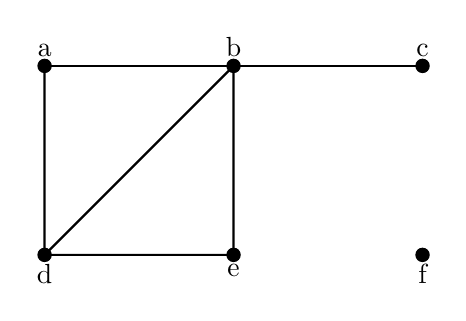
\begin{tikzpicture}[scale=1.2]
      \draw[fill=black] (1,1) circle (2pt);
      \draw[fill=black] (1,-1) circle (2pt);
      \draw[fill=black] (3,1) circle (2pt);
      \draw[fill=black] (3,-1) circle (2pt);
      \draw[fill=black] (5,1) circle (2pt);
      \draw[fill=black] (5,-1) circle (2pt);
      
      \node (a) [above] at (1,1) {a};
      \node (b) [above] at (3,1) {b};
      \node (d) [below] at (1,-1) {d};
      \node (e) [below] at (3,-1) {e};
      \node (c) [above] at (5,1) {c};
      \node (f) [below] at (5,-1) {f};
      
      \draw[thick] (1,1)--(3,1)--(5,1);
      \draw[thick] (1,1)--(1,-1)--(3,1)--(3,-1)--(1,-1);
    \end{tikzpicture}
  \end{center}


  \begin{itemize}
  \item \textbf{Number of vertices:} 6 $\{a,b,c,d,e,f\}$.
  \item \textbf{Number of edges:} 6
  \item \textbf{Degree of vertices:} 
    \begin{itemize}
    \item \textbf{degree(a):} 2
    \item \textbf{degree(b):} 4
    \item \textbf{degree(c):} 1
    \item \textbf{degree(d):} 3
    \item \textbf{degree(e ):} 2
    \item \textbf{degree(f ):} 0
    \end{itemize}
  \end{itemize}
  \qed
\end{document}
%%% Local Variables:
%%% mode: latex
%%% TeX-master: t
%%% End:
